\section{Line Detection}
\label{sec:lineDetection}

Many line detection algorithms stem from the road domain to detect lanes.
This is done for autonomous vehicles or safety systems for cars.
Most algorithms are trained on datasets like TuSimple \cite{tuSimpleDataset} or CULane \cite{cuLaneDataset}, which include images taken in the front view of cars.
While TuSimple is captured on US highways, CULane's images are taken in Beijing.
\autoref{fig:tusimpleExample} shows examples of TuSimple.

\vspace{0.8cm}

\begin{figure}[H]
    \centering
    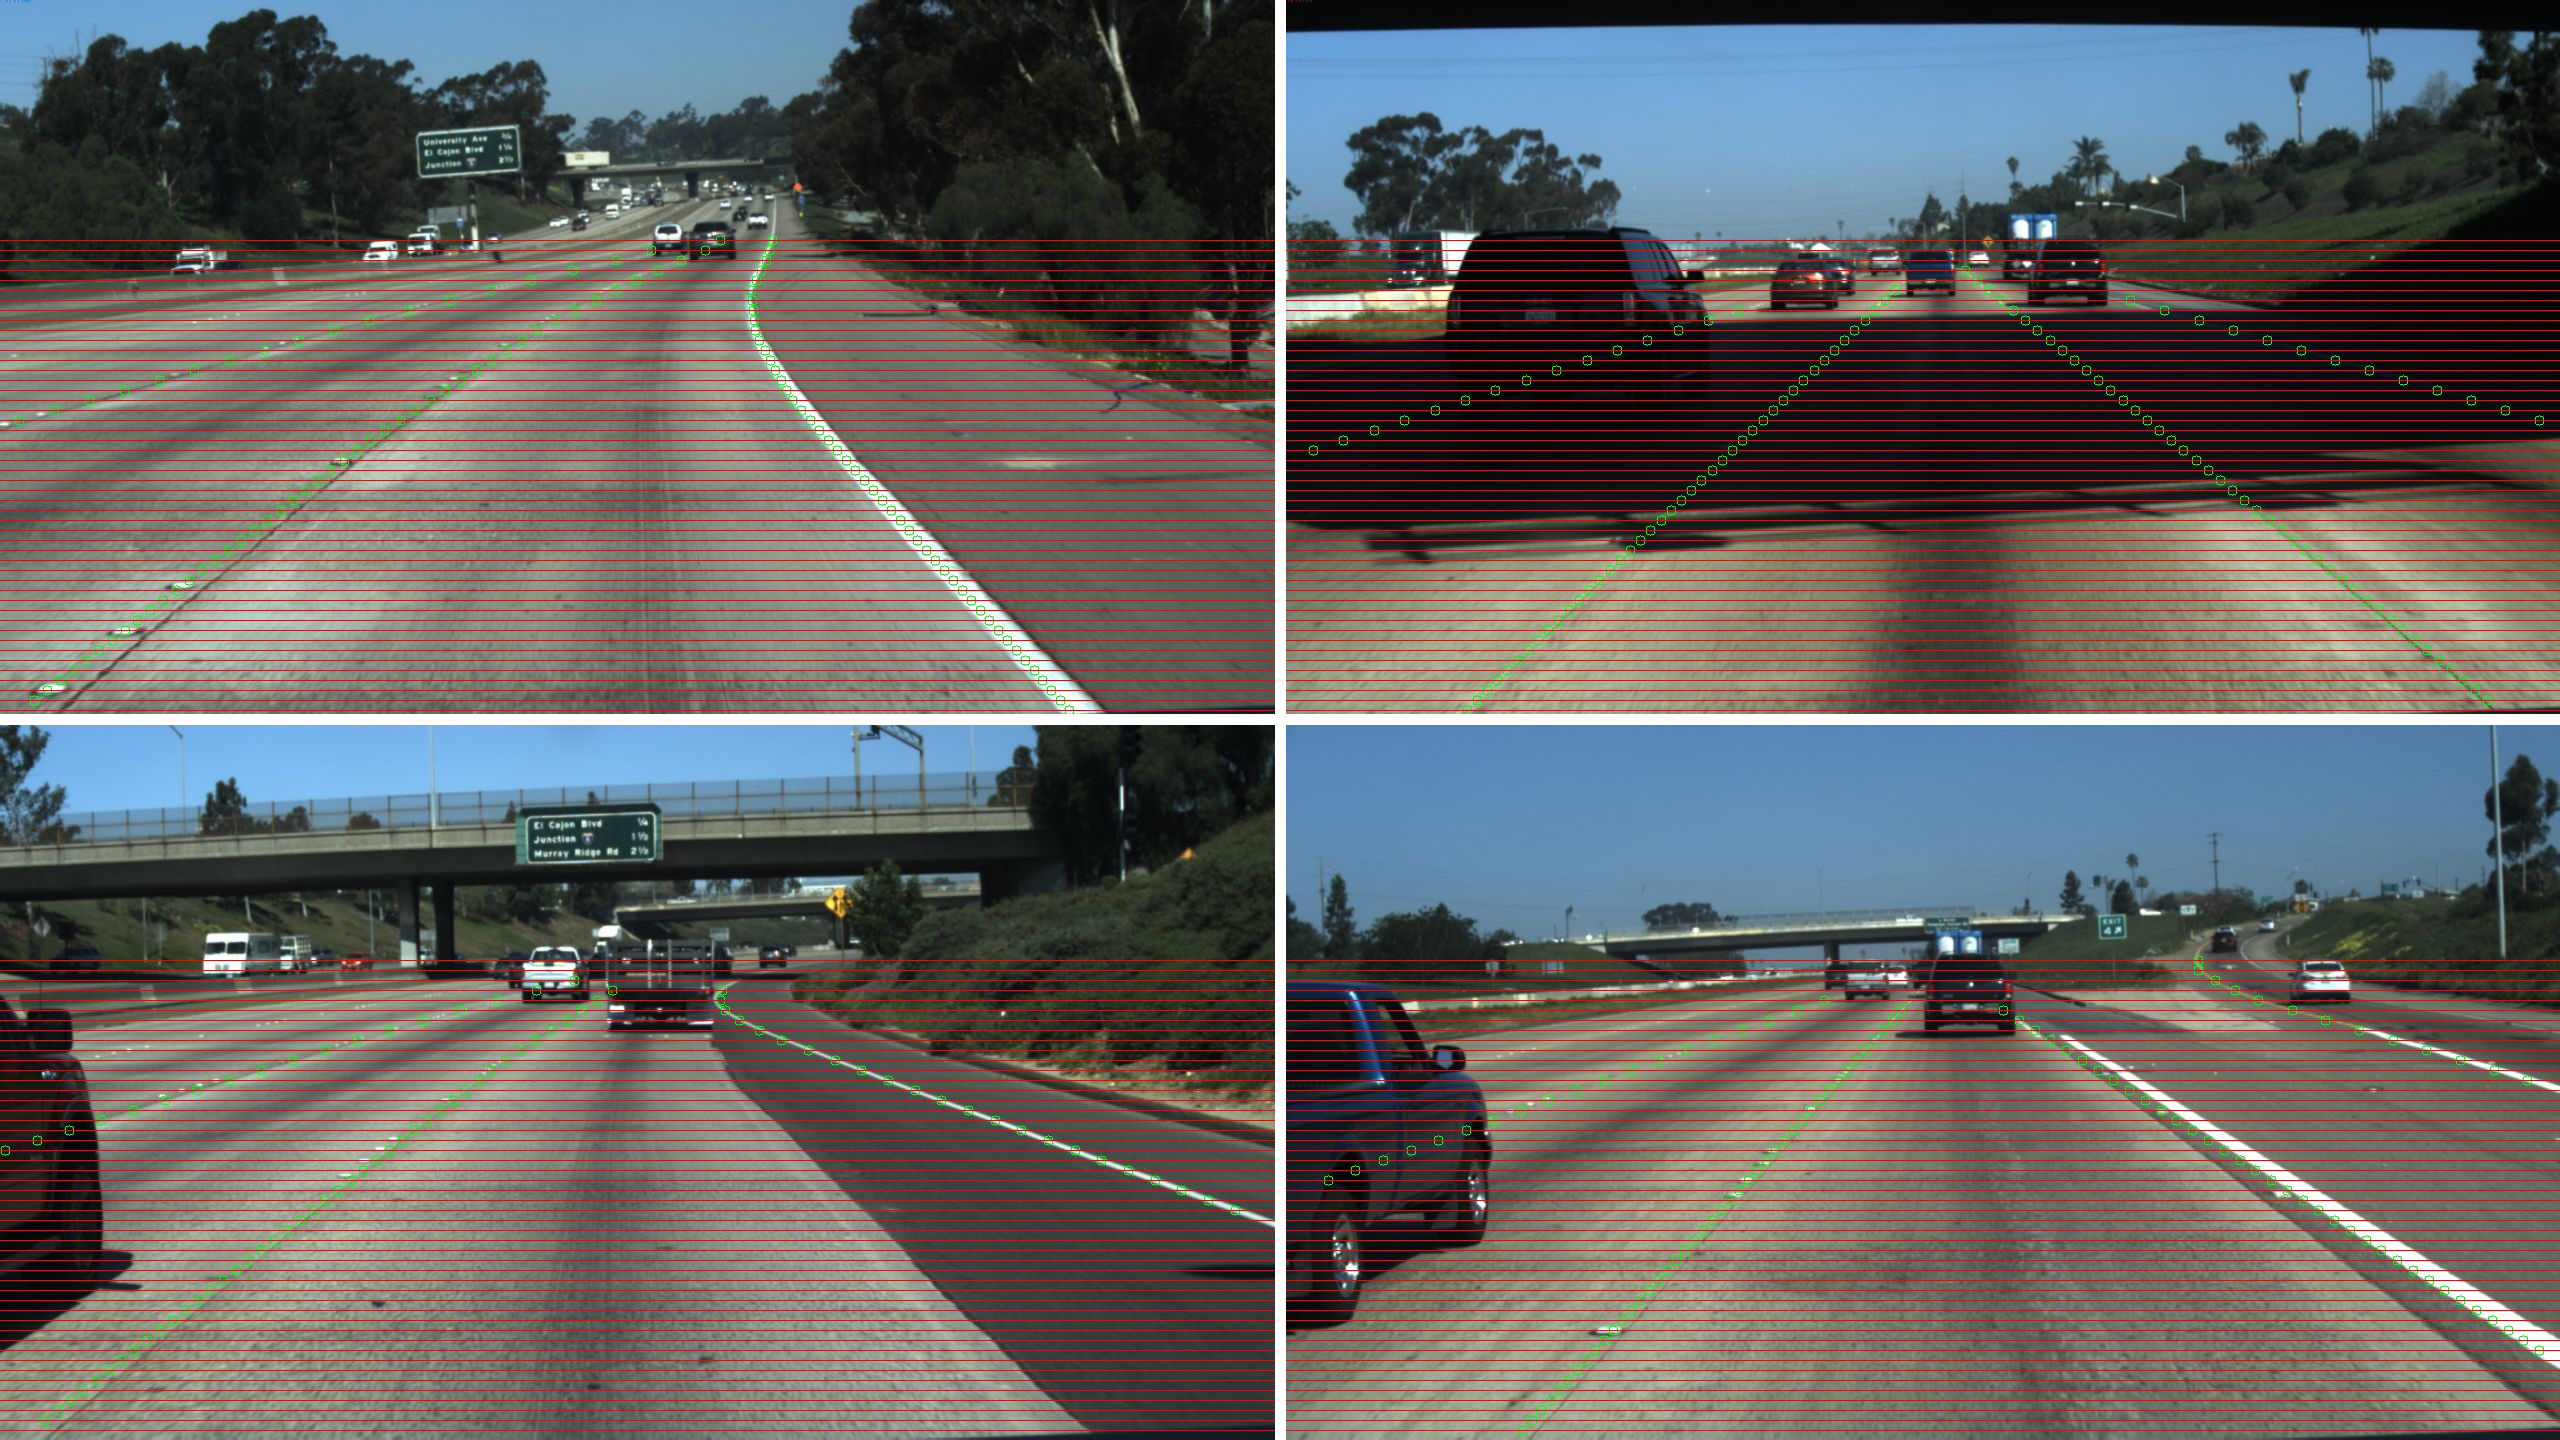
\includegraphics[width=\linewidth]{PICs/lineDetection/tusimple_example.jpg}
    \caption{Example images of TuSimple with annotations \cite{tuSimpleDatasetExampleImage}. Red lines are horizontal anchor lines. Green circles mark image coordinates, where road lanes and anchor lines intersect.}
    \label{fig:tusimpleExample}
\end{figure}

\vspace{0.8cm}

\noindent \cite{LaneDetectionCascadedCNNs2019} proposed one of the first lane detection approaches on TuSimple.
The proposed method detects lanes and classifies the kind of lane.
Two cascaded \ac{CNN}s are utilized; the first is an encoder-decoder network, for instance, segmentation, and the second is a classification network.
\cite{rowwiseClassification2020} uses an encoder-decoder network at the start, then an introduced horizontal reduction module that transforms features into a row-wise representation. In the last stage, the network outputs two branches. One that predicts the horizontal location of lanes and another that outputs a confidence score.
However, both approaches utilize encoder-decoder structures and are similar to the techniques used for semantic segmentation.
Other structures for lane detection include key point extraction, grid systems, or polyline regression.
The following three paragraphs describe research in those directions, following projects with similar approaches for the rail domain.

\subsubsection{Keypoint Detection on the Road}

\cite{LineCNN2020} proposed Line-CNN, which includes a ResNet backbone and an introduced "Line Proposal Unit".
The model suggests a series of lines to locate road lanes.
After the proposal, the line with the highest confidence score is fitted with horizontal offsets to match the actual lane.
Similar to Line-CNN, the method introduced in \cite{KeepEyesOnLane2021} also proposes lines with confidence scores and fits the resulting output with horizontal offsets.
The innovative aspect of this approach lies in introducing an anchor-based attention mechanism.
This added module results in higher accuracy and a much faster model with speeds up to 250 \ac{FPS}.
\cite{CurveLaneNAS2020} proposed a network that predicts road lanes with horizontal offsets from a pre-defined vertical anchor.
A \ac{NAS} is also utilized to find the optimal architecture for this task.
Another approach that uses key points is introduced in \cite{GANet2022}.
This architecture utilizes a "Lane-aware Feature Aggregation Module" to strengthen the connection between neighboring key points and achieves state-of-the-art performance.

\subsubsection{Grid System}

An approach that uses grid systems is proposed by \cite{laneDetectionGrid2020}.
Here, a row-wise classification is performed for a predefined number of grids.
The number of grids is equivalent to the number of lanes that can be detected.

\subsubsection{Polyline Regression}

A regression approach is proposed in \cite{PolyLaneNetRoad2021} that predicts the polynomials of lanes.
ResNet and EfficientNet backbones extract features, which are then used to forecast lines.
Each line includes the coefficients of a polynomial, a starting parameter, and a confidence score.
Additionally, a shared horizon line is predicted, where all polylines end.
Compared to other state-of-the-art approaches, \cite{PolyLaneNetRoad2021} proposes a computationally efficient method with speeds up to 115 \ac{FPS}.
While accuracy is lower than with other methods, it still is comparable.
\cite{DetectingLanesWithBezierCurves2023} proposed an approach that also predicts the parameters of a cubic curve.
Instead of the polynomial coefficients, the parameters of Bezier curves are predicted.
A Bezier curve is fitted in an area defined by four control points.
A typical backbone like ResNet with additional feature flip fusion modules is utilized for the network structure.
Then, a pooling and two convolutional layers are implemented sequentially, which form the final output of predictions.
Compared to polynomial fitting, the approach proposed in \cite{DetectingLanesWithBezierCurves2023} is superior.

\subsubsection{Rail Domain}

Even though much has been done in the road domain, and the rail domain is usually not considered, some research has still been conducted to adapt lane detection algorithms for trains.
Some of the mentioned research approaches utilize key point extraction to detect rails.
\cite{topologyGuidedRailDetection2022} detects rails by adapting the concept of key point extraction with semantic segmentation as pre-processing.
The technique can be divided into four stages.
In the first stage called "image preprocessing", a semantic segmentation network filters out the rails in an image.
An inverse perspective transformation is utilized to bring the binary mask into a bird-eye view for easier image handling in further steps.
The second stage, "rail-track discretization", includes a key point extraction, connectivity judgment and breakpoint connection modules to divide the one-class segmentation mask into different rails.
The third stage consists of the "rail lane reconstruction", where the data from the second step is combined with the bird-eye view from the first to connect the extracted key points. Resulting in a complete rail lane instead of discrete points.
In the final stage, rails are matched in pairs for the final output.
However, no distinction is made between the train's rail and other rails.
Two additional issues lay in the complex data processing of this approach.
On the one hand, it is stated that the algorithm's accuracy relies too much on the semantic segmentation used at the start.
On the other hand, no records of speed are available.
Due to the intricacy of the proposed approach, the complex and cascaded algorithms could easily exceed real-time requirements.

%\vspace{1cm}

Another state-of-the-art approach to filtering out rails is to divide the output into grids \cite{li2022rail}.
This technique is adapted from the road domain from \cite{laneDetectionGrid2020}.
Each rail is predicted in a separate grid, and the number of rails is predefined with the hyperparameter $C$, as shown in \autoref{fig:gridLineDetection}.
A row-wise classification problem is solved in each grid, where the target class corresponds to the cell that encompasses the target rail.
After that, the predicted cells are translated into image coordinates to calculate the final output.
The architecture is shown in \autoref{fig:gridLineDetection}.
The output image shows the focus on detecting all rails in an image.
This approach relies only on the feature extractor and does not need a decoder.
In 2024, this approach is also used by TEP-Net \cite{tepNet2024} with only the train's own two rails ($C=2$) for state-of-the-art comparison.

\begin{figure}[H]
    \centering
    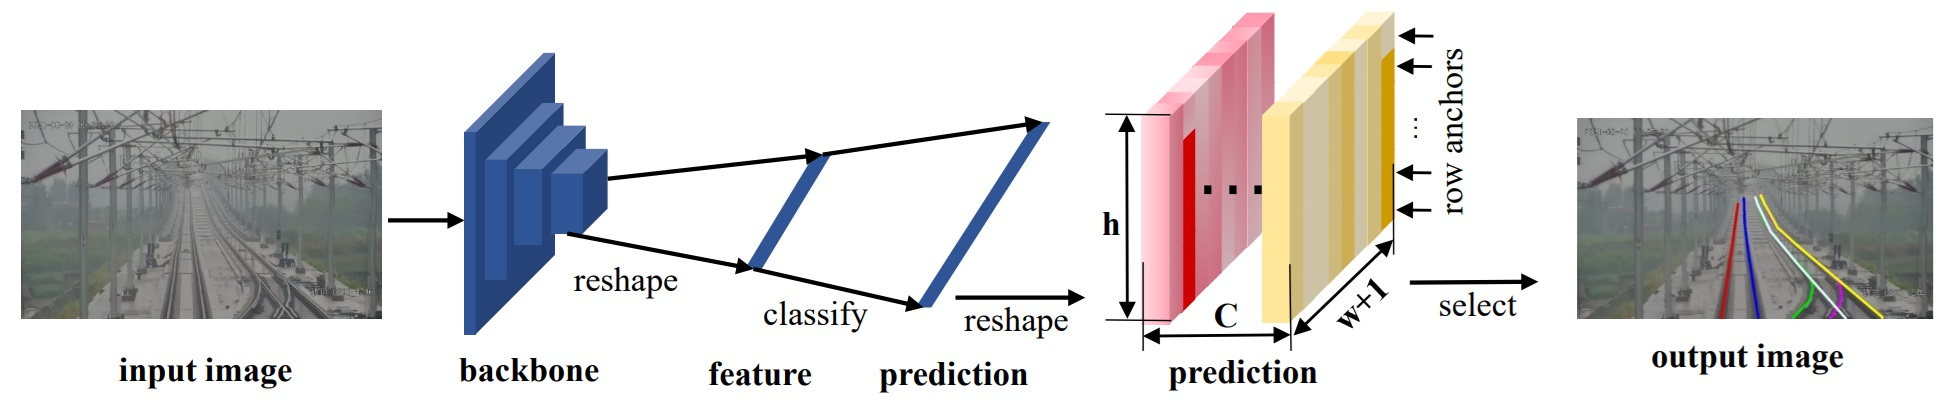
\includegraphics[width=\linewidth]{PICs/lineDetection/gridDetection.jpg}
    \caption{Rail detection with Gridsystem \cite{li2022rail}. Hyperparameters: $C$ is the number of rails (number of grids). $h$ is the number of vertical cells. $w+1$ is the number of cells horizontally with an additional column for a background class when no rail is detected in a row.}
    \label{fig:gridLineDetection}
\end{figure}

\noindent \ac{TEP}-Net \cite{tepNet2024} introduces another regression approach.
\cite{RailraodSemanticPossibleTracks2020} and \cite{TPENet2023} expect that switch states cannot accurately be determined.
Therefore, they try to filter out all possible tracks.
\cite{tepNet2024} extends the problem formulation, assuming that switch states can be correctly predicted.
This eliminates the need for heavy postprocessing and leads to a lightweight model that only predicts the right and left rail of the train's path.
Since the use case of \cite{tepNet2024} and the goal of this work overlap in almost all aspects, this paper is described in more detail in \autoref{sec:baselinepaper}.